% Generated by figures/make_paper_figures.py

\begin{figure}[t]
  \centering
  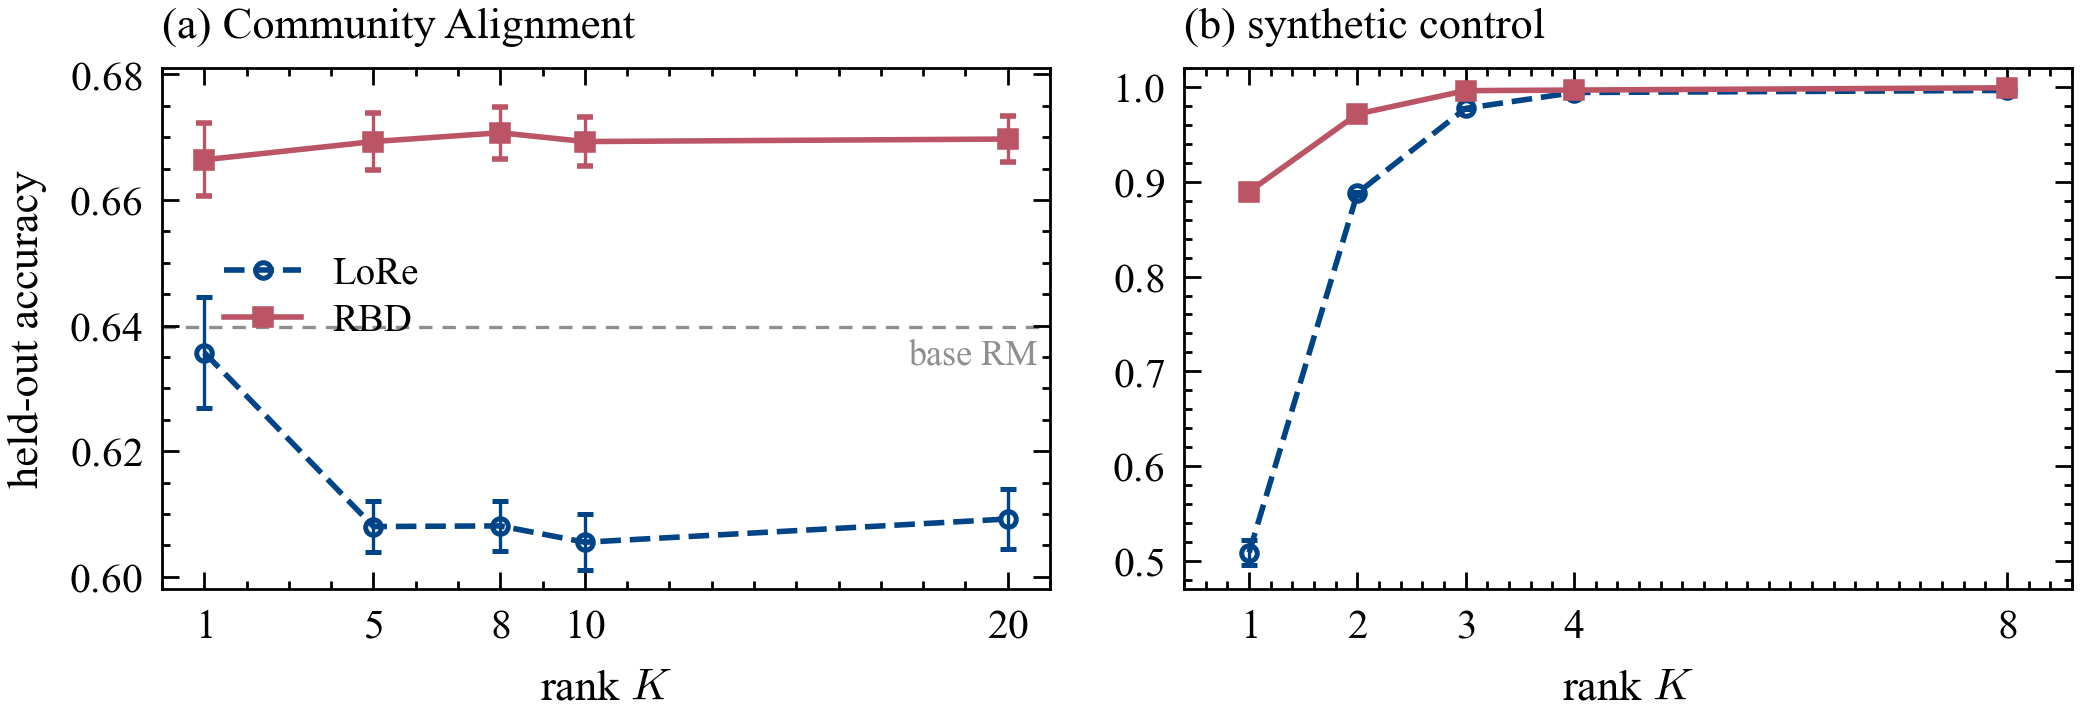
\includegraphics[width=\linewidth]{figures/fig_rank_panels.png}
  \caption{Held-out accuracy against rank. On Community Alignment (a) RBD sits above the
  pretrained reward head at every rank while LoRe sits below it, and the separation is flat
  in $K$. On the synthetic control (b) the ordering is the same but the margin is far larger
  at low rank: RBD at $K=1$ matches LoRe at $K=2$, which is what the simplex constraint
  costs, and both saturate by $K=3$--$4$ where the dataset is near-ceiling by construction.
  Error bars are one standard deviation over five seeds (a) and three seeds (b).
  Tables~\ref{tab:ca-headline} and~\ref{tab:synth-rank}.}
  \label{fig:rank-panels}
\end{figure}

\begin{figure}[t]
  \centering
  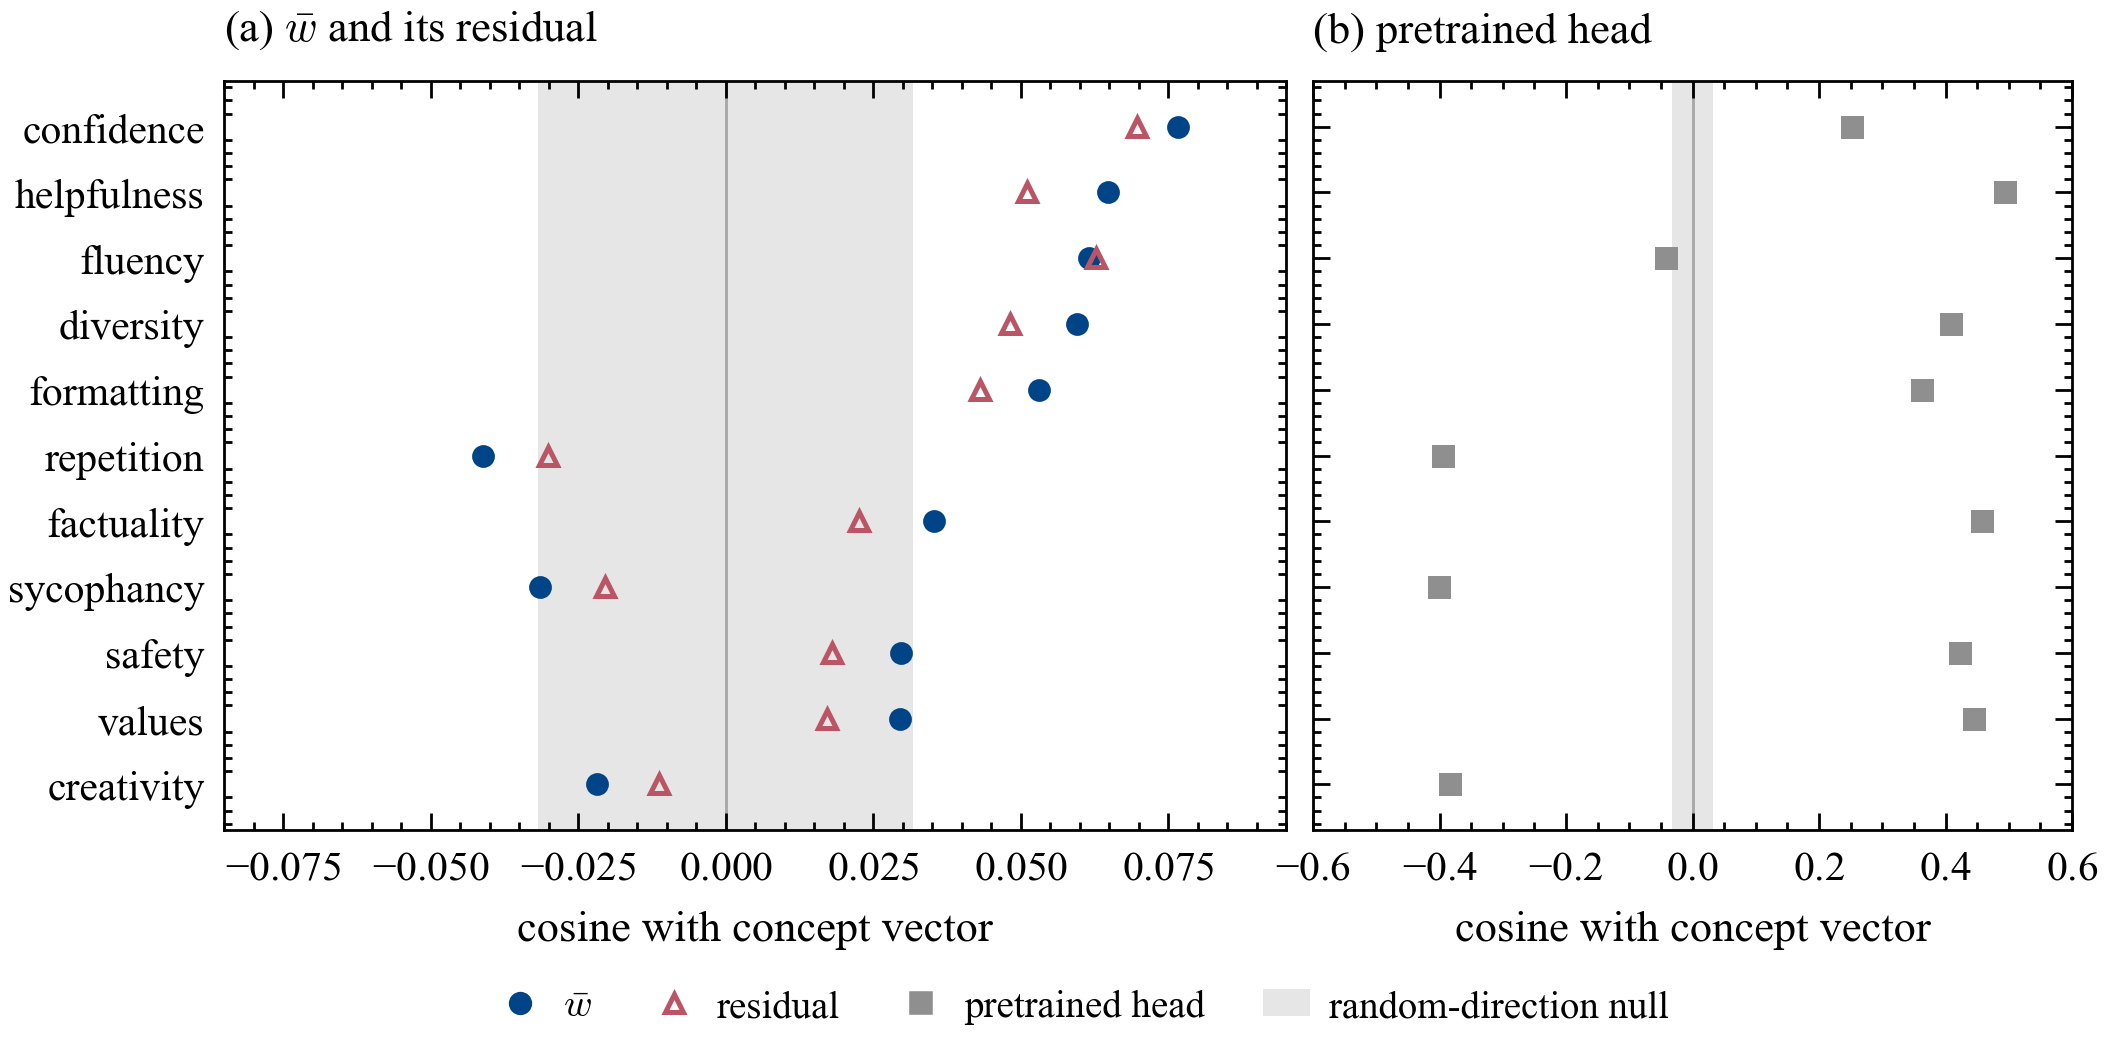
\includegraphics[width=\linewidth]{figures/fig_concepts.png}
  \caption{Cosine alignment of the population direction with named concepts, against a
  random-direction null (shaded, $|\cos| < 0.0318$; 10{,}000 draws). A point outside the band
  is significant. (a) $\bar{w}$ clears the null on seven of eleven concepts, but its residual
  after removing the component along the pretrained head clears only five, so most of the
  alignment is inherited rather than learned. \texttt{fluency} is the exception: its residual
  exceeds $\bar{w}$'s own cosine and runs opposite in sign to the head's. (b) The pretrained
  head clears the null on all eleven, on an axis an order of magnitude wider.
  Table~\ref{tab:concepts}.}
  \label{fig:concepts}
\end{figure}

\begin{figure}[t]
  \centering
  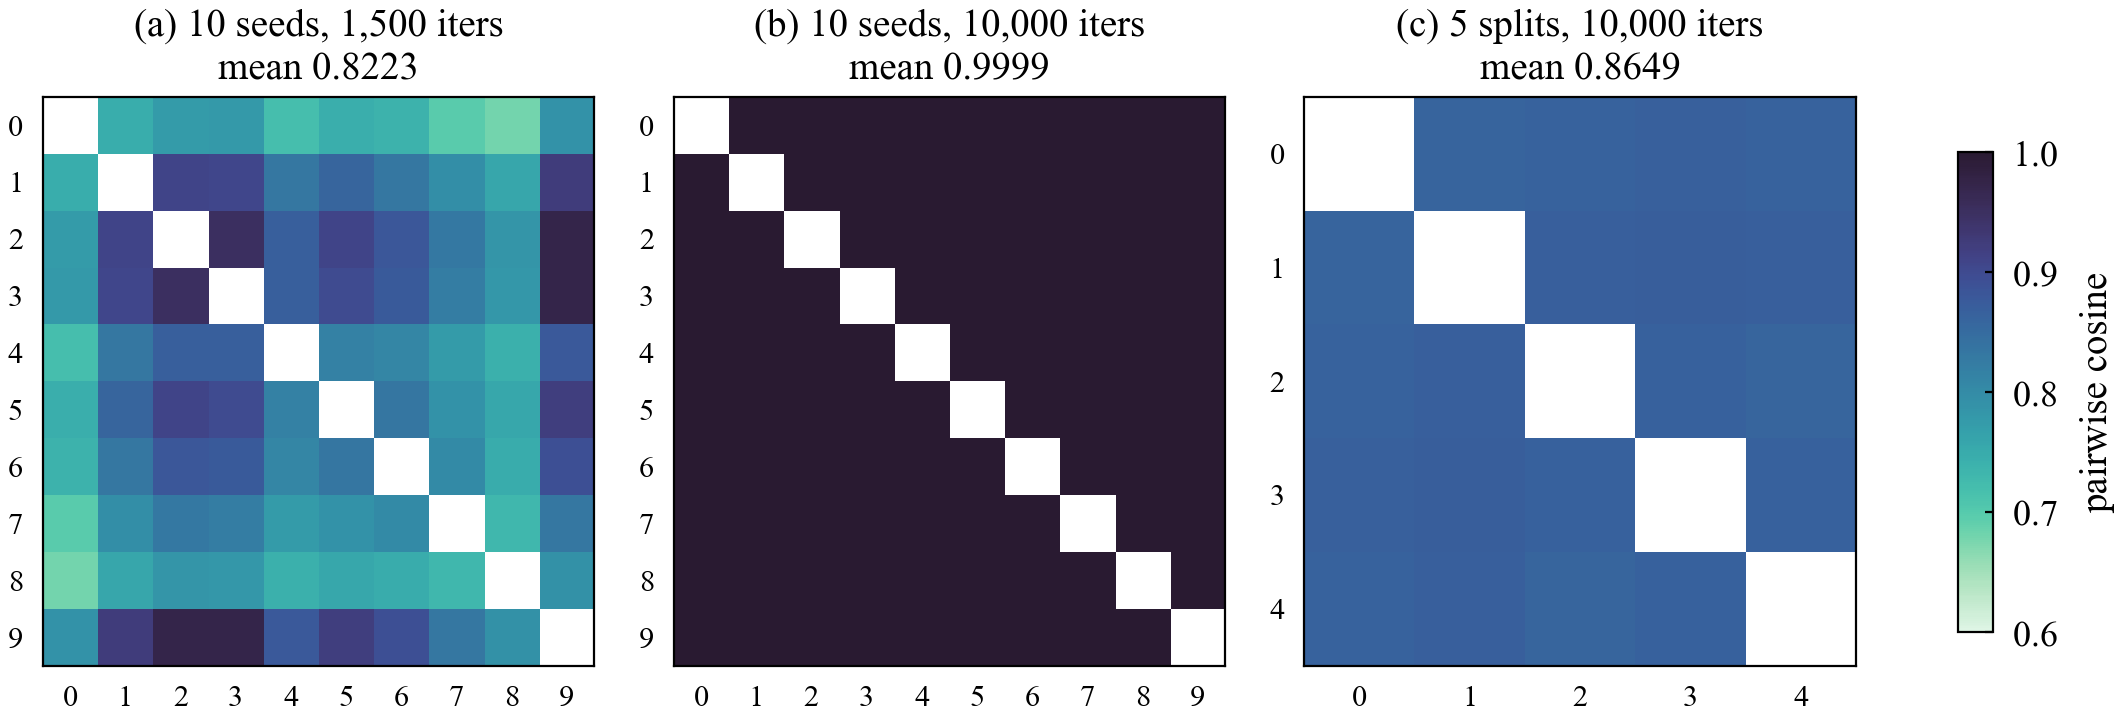
\includegraphics[width=\linewidth]{figures/fig_stability.png}
  \caption{Pairwise cosine between population directions $v_{\mathrm{pop}}$ from independent
  runs. At 1{,}500 iterations (a) the spread across seeds looks like a flat optimum with many
  solutions; at 10{,}000 iterations (b) it collapses to $0.9999$, so the apparent instability
  was undertraining rather than degeneracy. Re-drawing the train/test split (c) still moves
  the direction ($0.8649$), which is a property of the data rather than of the optimiser.
  Table~\ref{tab:stability}.}
  \label{fig:stability}
\end{figure}
